\section{The Hilbert's theorem}
\begin{theorem}[Hilbert's theorem]
    Let \(S\) be a complete and simply connected regular surface with
    Gaussian curvature \(K=-1\), then there is no isometric embedding of
    \(S\) into \(\mathbb{R}^3\).
\end{theorem}
\begin{proof}[Sketch of proof]
    \begin{enumerate}[(1)]
        \item \((S,g)\) is isometric to the hyperbolic plane in 
        \(\mathbb{H}^2\)\\
        \(\Rightarrow\) \(Area(S)=Area(\mathbb{H}^2)=+\infty\).
        \item If \(\exists\) an isometric embedding \(
            \varphi\colon S\to \mathbb{R}^3\), then we can construct a 
            global parametrization of \(S\) with coordinate curves being
            asymptotic lines, and the parametrization forms a
            ``chebyshev net'' such that any quadrilateral of coordinate
            curves has area \(<2\pi\). This implies 
            \[Area(S)<2\pi.\]
    \end{enumerate}
    Then (1) and (2) yields a contradiction.
\end{proof}
\begin{definition}
    A local parametrization \(\phi (u,v)\colon U\subset \mathbb{R}^2\to
    S\) is called a ``chebyshev net'' if the length of opposite sides of
    any quadrilateral formed by coordinate curves are equal.
\end{definition}
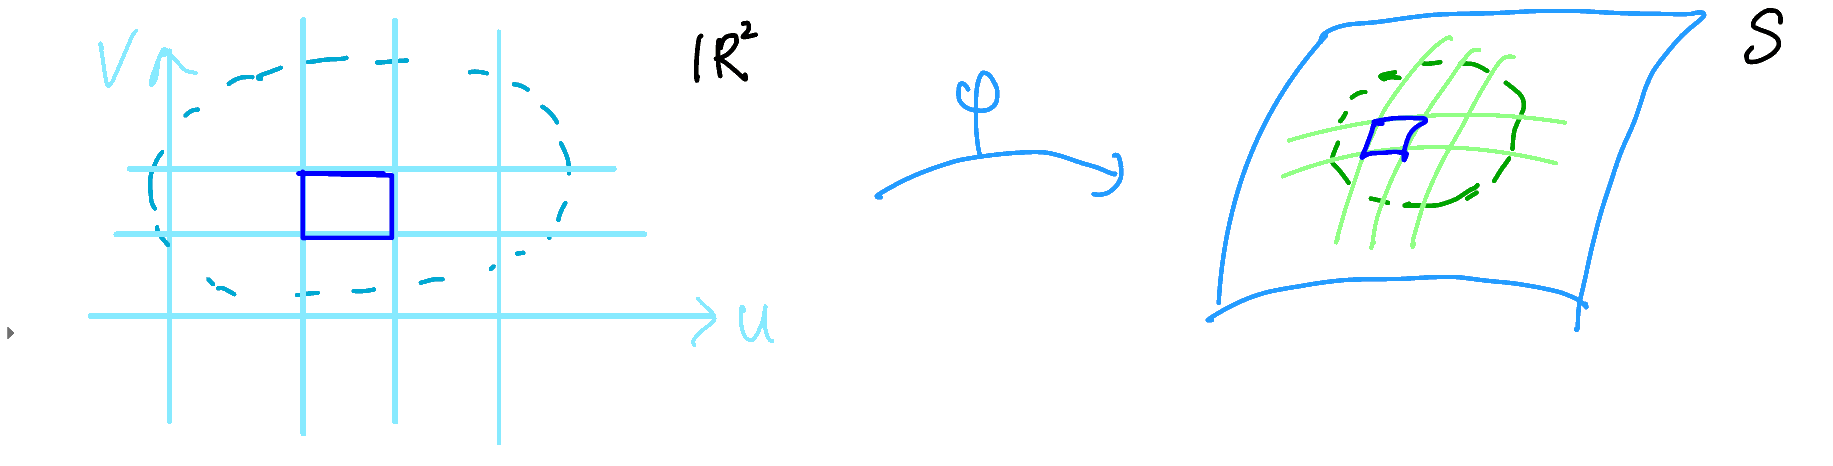
\includegraphics[scale=0.4]{picture/week15/chebyshev net.png}
\begin{proof}[proof of (1)]
    First, from the minding's theorem, we know \(S\) and \(\mathbb{H}\)
    are locally isometric to each other. Let \(p\in S\), \(p'
    \in \mathbb{H}\), the local isometry yields a linear isometry
    \(l\colon T_p S\to T_{p'} \mathbb{H}\).

    To construct a global isometry, let's consider
    \begin{center}
        \begin{tikzcd}
            T_p S \arrow[d, "\exp_p"] \arrow[r, "l"] & T_{p'}\mathbb{H} \arrow[d, "\exp_{p'}"] \\
            S \arrow[r, dashed]                      & \mathbb{H}                             
        \end{tikzcd}
    \end{center}
    By the Hadamard theorem \(\rightarrow\) \(\exp_p\) and \(\exp_{p'}\)
    are diffeomorphism.
    \footnote{
        Hadamard's theorem: let \((M,g)\) be a complete Riemannian manifold
        with \(K_M\le 0\), where \(K_M\) is the sectional curvature, then
        \(\exp_p\colon T_p M\to M\) is a covering map. Moreover, if \(M\)
        is simply connected, then \(\exp_p\) is a diffeomorphism.
    }
    Hence \(f=\exp_p\circ l\circ \exp_{p'}^{-1}\colon S\to \mathbb{H}\)
    is a diffeomorphism. We can further conclude that \(f\) is a local 
    isometry. This follows from the Cartan's theorem:
    \begin{itemize}
        \item Let \((M,g)\), \((M',g')\) be two Riemannian manifolds, 
        \(p\in M\), \(p'\in M'\).
        \item Let \(l\colon T_p M\to T_{p'}M'\) be a linear isometry
        \item \(U\) is a normal neighborhood of \(p\) on which \(\exp_p\)
        is a diffeomorphism.
        \item \(\forall V\in T_q M\), and let \(P_t\) be the parallel transport
        along \(\gamma(t)\), then \(P_t^{-1}(V)\) is a vector in \(T_p M\).
        The linear isometry yields \(l\circ P_t^{-1}(V)\) to be a vector
        in \(T_{p'}M'\). Let \(q'=\exp_{p'}\circ l\circ\exp_{p}^{-1}q
        \in M'\), \(\gamma'(t)\) is the geodesic from \(p'\) to \(q'\)
        and \(P_t'\) is the parallel transport along \(\gamma'(t)\).
        Then using \(P_t '\), we get a vector \(P_t'\circ l\circ 
        P_t^{-1}(V)\\in T_{q'}M'\)
        \(\Rightarrow L_t=P_t'\circ l\circ P_t^{-1}\colon T_q M\to
        T_{q'}M'\) is a linear isometry. If \(\forall\) vectors 
        \(X, Y,Z,W\in T_q M\) we have
        \[
            R(X,Y,Z,W)=R'(L_t(X),L_t(Y),L_t(Z),L_t(W))    
        \]
        then \(f=\exp_{p'}\circ l\circ \exp_p^{-1}\) is a local isometry.
        \begin{center}
            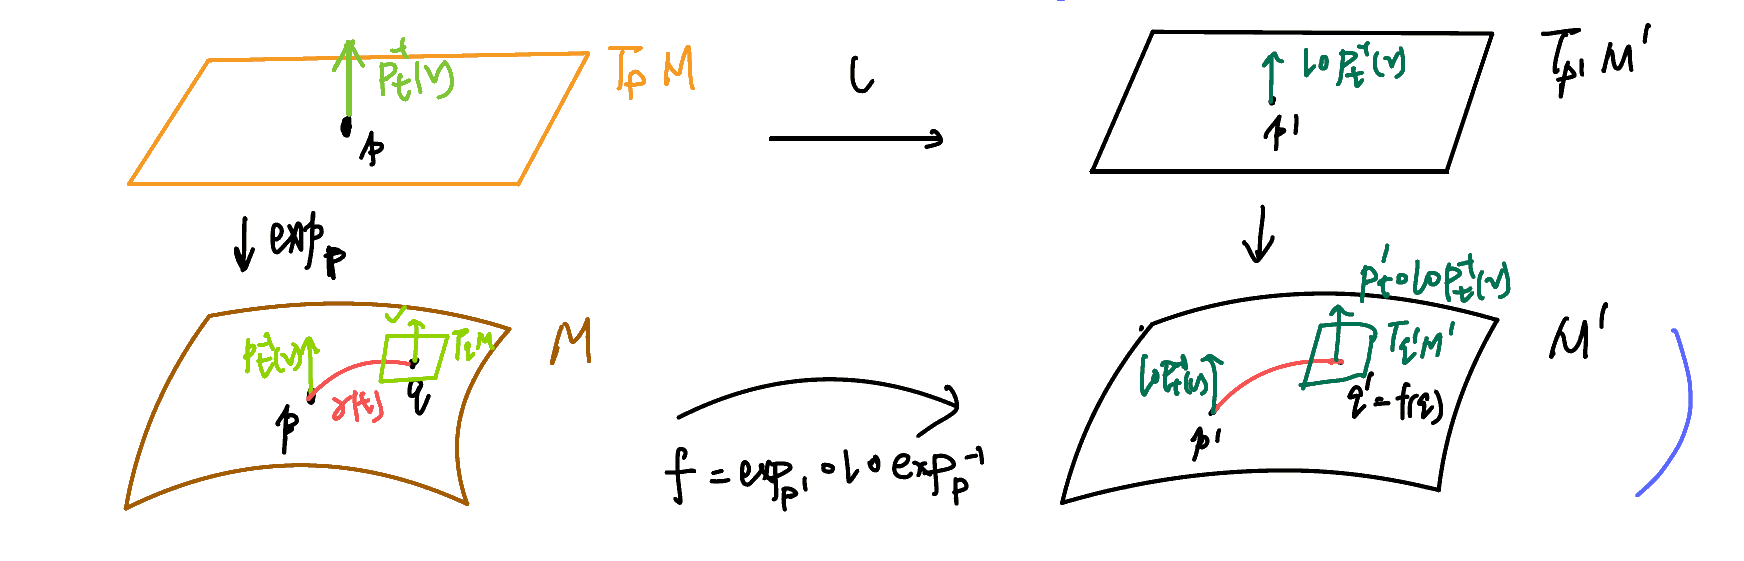
\includegraphics[scale=0.4]{picture/week15/cartan theorem.png}
        \end{center}
    \end{itemize}
    Hence, we see \((S,g)\) and \(\mathbb{H}\) are isometric to each other on
    \(\mathbb{H}^2\). We consider geodesic polar coordinate such that
    \[ds^2=dr^2+\left(\sinh r\right)^2 d\theta^2.\]
    Then the radial geodesic \(\gamma(t)=\exp_p(t\pdv{r})\) defines for all
    time \(t\), \(\Rightarrow t\in (0,+\infty)\)
    \[Area(S)=Area(\mathbb{H})=\int_{0}^{2\pi} \int_{0}^{+\infty}
    \sinh r drd\theta=+\infty\]
\end{proof}
\begin{proof}[proof of (2)]
    Now we assume \(S\) is isometrically embedded into \(\mathbb{R}^3\).

    \underline{Claim 1}: \(\forall p\in S\), \(\exists\) local parametrization
    \((s,t)\) of \(S\), such that the \engordnumber{1} and 
    \engordnumber{2} fundamental form are given by
    \[
      I=ds^2+2\cos \alpha ds dt +dt^2  
    \]   
    \[\II=2\sin\alpha ds dt\]
    where \(\alpha=\alpha(s,t)\) satisfies the Sine-Gordan equation
    \[\alpha_{st}=\sin \alpha,\quad 0<\alpha<\pi\]
    From this expression of I and II, we see
    \begin{enumerate}[(1)]
        \item the length of opposite sides of coordinate quadrilateral
        are the same \(\Rightarrow\) \((s,t)\) forms a chebyshev net,
        \(\alpha\) is the angle between \(s\)-curve and \(t\)-curve.
        \begin{center}
            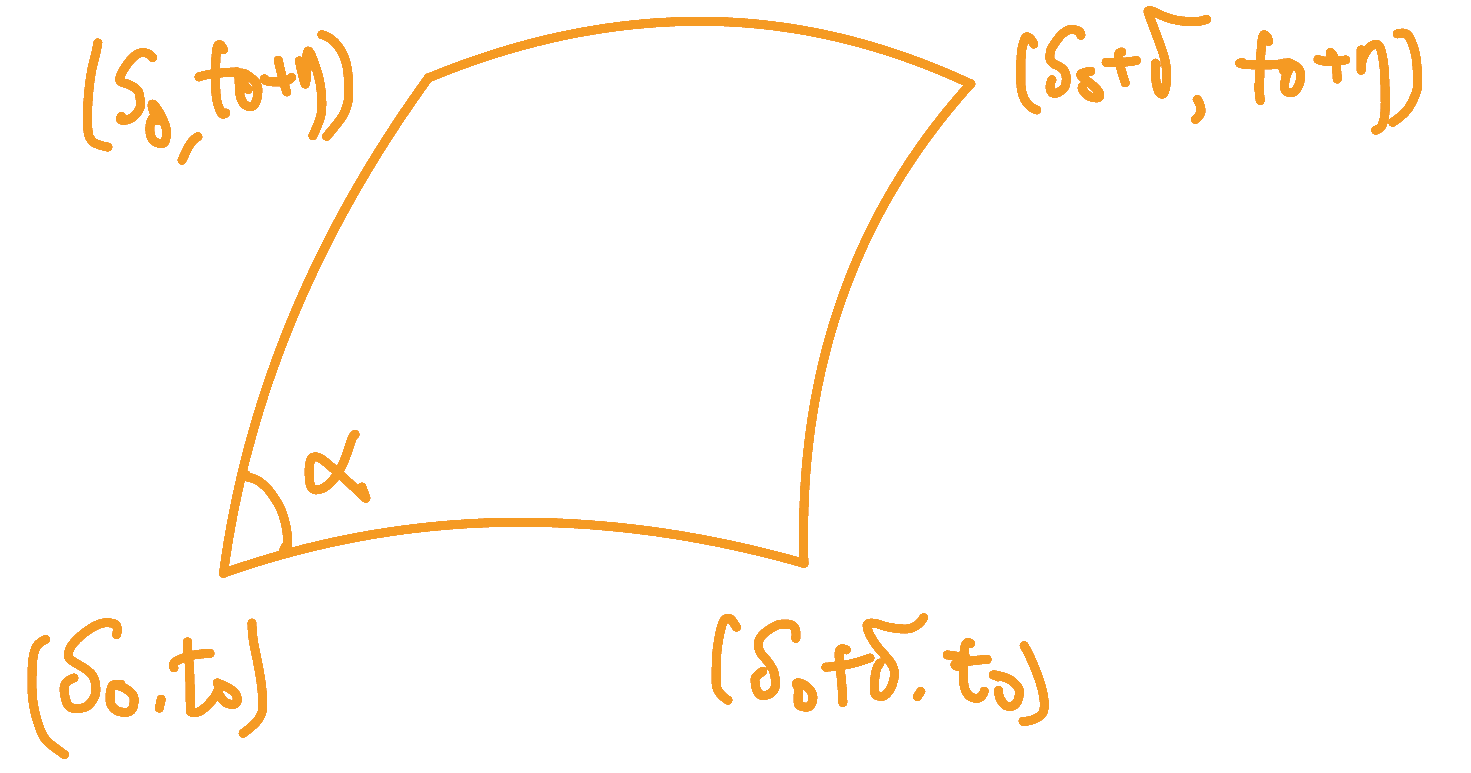
\includegraphics[scale=0.2]{picture/week15/quadrilateral.png}
        \end{center}
        \item coordinate \(s\)-curve and \(t\)-curve are asymptotic lines
    \end{enumerate}
    \begin{proof}[Proof of claim 1]
        \(K=-1\) on \(S\) \(\Rightarrow\) all pairs are umbilical.
        Hence, we can first choose local parametrization \(x^1,x^2\)
        such that 
        \[I=g_{11}(dx^1)^2+g_{22}(dx^2)^2\]
        \[II=h_{11}(dx^1)^2+h_{22}(dx^2)^2\]
    \(\Rightarrow\) principal curvatures \(k_1=\frac{h_{11}}{g_{11}},
    k_2=\frac{h_{22}}{g_{22}}\).
    The codazzi equation is 
    \[\frac{\partial_2k_1}{k_2-k_1}=\partial_2 \log \sqrt{g_{11}}\]
    \[\frac{\partial_1k_2}{k_1-k_2}=\partial_1 \log \sqrt{g_{22}}\]
    Since \(k_1k_2=-1\), we set 
    \[
        k_1=\tan\theta,\quad k_2=-\cot\theta,\quad 0<\theta<\frac{\pi}{2}    
    \]
    \(\Rightarrow k_1-k_2=\tan\theta+\cot \theta=
    \frac{1}{\sin\theta\cos\theta}\).
    Then the codazzi equation 
    \end{proof}
\end{proof}
